\documentclass{article}
\usepackage[a4paper, textwidth=180mm, textheight=260mm]{geometry}
\usepackage[hidelinks, colorlinks=true]{hyperref}
\usepackage{graphicx}
\usepackage{booktabs}
\usepackage{tikz}

% Configurations
\setlength{\parindent}{0pt}
\pagestyle{empty}

% Symbols
\newcommand{\symbolHt}{1.2em}
\newcommand{\phoneChar}{
    \begingroup\normalfont
    \raisebox{-0.08cm}{ % '%' for no space in end
        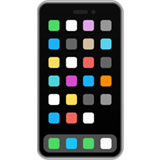
\includegraphics[height=\symbolHt]{icons/phone.png}}%
    \endgroup
}
\newcommand{\homeChar}{
    \begingroup\normalfont
    \raisebox{-0.05cm}{
        
\includegraphics[height=\symbolHt]{icons/house.png}}
    \endgroup
}
\newcommand{\githubChar}{
    \begingroup\normalfont
    % From: https://www.flaticon.com/free-icon/github_2111432?term=github&page=1&position=4&origin=search&related_id=2111432
    \raisebox{-0.07cm}{
        
\includegraphics[height=\symbolHt]{icons/github.png}}
    \endgroup
}
\newcommand{\webChar}{
    \begingroup\normalfont
    % From: https://www.flaticon.com/free-icon/world-wide-web_1006771?term=website&page=1&position=1&origin=search&related_id=1006771
    \raisebox{-0.07cm}{
        
\includegraphics[height=\symbolHt]{icons/world-wide-web.png}}
    \endgroup
}
\newcommand{\linkedinChar}{
    \begingroup\normalfont
    % From: https://www.flaticon.com/free-icon/linkedin_3536505?term=linkedin&page=1&position=1&origin=search&related_id=3536505
    \raisebox{-0.07cm}{
        
\includegraphics[height=\symbolHt]{icons/linkedin.png}}
    \endgroup
}
% New section
\newcommand{\newsec}[1]{
    {\bf \large #1}
    \vspace{2mm}
    \hrule
    \vspace{2mm}
}
% New experience header
\newcommand{\expheader}[3]{
    {\bf #1} \hfill {\it #2} \hfill #3
}
% New education header
\newcommand{\eduheader}[4]{
    {\bf #1} \hfill {\it #2} \hfill #3 \hfill \\
    {\bf #4}
}

\begin{document}
    \begin{center}
        {\bf \LARGE Avneesh Mishra} \\ [4mm]
        \phoneChar +91 99163 32393 \qquad
        \texttt{123avneesh@gmail.com} \qquad
        \homeChar Bengaluru, Karnataka, IN \\ [1mm]
        \linkedinChar \href{
            https://www.linkedin.com/in/avneesh-mishra/}{
            avneesh-mishra} \qquad
        \githubChar \href{https://github.com/TheProjectsGuy}{
            TheProjectsGuy} \qquad
        \webChar \href{https://theprojectsguy.github.io/}{
            theprojectsguy.github.io}
    \end{center}
    % --------------------- Main profile ---------------------
    \newsec{Profile}
    A Mechatronics engineer with research experience in computer 
    vision, AI \& robotics. Skilled at writing maintainable code and 
    leveraging cutting-edge developments to achieve project goals.
    \\ [4mm]
    % ----------------- Areas of experience -----------------
    \newsec{Areas of Experience}
    \begin{tabular}{cp{0.9\textwidth}}
        \raisebox{-0.8cm}{
        \tikz \fill [green, draw=black] (0.0,0.0) rectangle (0.2,1);
        } & % ------ Strong suits ------
        Computer Vision (Image Retrieval \& Matching, VPR, SLAM
        systems) - AI (PyTorch, TensorFlow, WandB) - Computer Science
        (Linux, MacOS, Windows; Docker; OS \& Hardware) - Programming
        (Python, C++, Bash/Shell) - Frameworks (Pandas, ROS) \\ [1mm]
        \raisebox{-0.8cm}{
        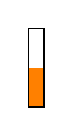
\begin{tikzpicture}
            \fill [orange] (0.0,0.0) rectangle (0.2, 0.5);
            \draw[black] (0.0,0.0) rectangle (0.2,1);
        \end{tikzpicture}
        } & % ------ Weak suits ------
        Systems Administration (HPC, IAM, NAS, Networking, Storage,
        Hardware) - Cloud (AWS) - Application Development (Python,
        Web, Unity AR) - Programming (MATLAB, Javascript, Swift) - CAD
        (Electronics: KiCAD; Mechanical: Fusion 360, SolidWorks) 
        \\ [1mm]
        & {\bf Hobbies:} Reading, finance, cooking
    \end{tabular}
    \\ [4mm]
    % ------------------------ Education ------------------------
    \newsec{Education}
    \expheader{M.S. by Research (CSE)}{\href{
        https://robotics.iiit.ac.in/}{Robotics Research Center} (RRC), 
        IIIT Hyderabad}{August 2021 to Present}{}
    \begin{itemize}
        \setlength{\itemsep}{0mm}
        \item SLAM (Simultaneous Localization and Mapping) using 
            cameras, VPR systems, local features matching, global
            image descriptors.
        \item RRC Summer School 2022 - Multi-View Geometry (\href{https://github.com/TheProjectsGuy/RRC22-Summer-School-MVG4}{GitHub})
        \item Student SysAdmin (from May 2022 to Feb 2023)
        \item First year {\bf GPA 10/10}
    \end{itemize}
    \expheader{B.Tech. in Mechatronics Engineering}{Manipal Institute 
        of Technology}{July 2016 to July 2020}
    \begin{itemize}
        \setlength{\itemsep}{0mm}
        \item Minor in Robotics
        \item Gold medalist in the batch (with {\bf CGPA 9.88/10})
    \end{itemize}
    % ----------------------- Experience -----------------------
    \newsec{Experience}
    \expheader{Consultant}{
        \href{https://artpark.in/}{Artpark}, RBCCPS, IISc Bangalore}{
        March 2021 to August 2021}
    \begin{itemize}
        \setlength{\itemsep}{0mm}
        \item Teleoperation using Asha (\href{
            https://www.hansonrobotics.com/sophia/}{Sophia} from 
            Hanson Robotics) with Team Aham for the \href{
            https://avatar.xprize.org/prizes/avatar}{ANA Avatar 
            XPrize} challenge.
        \item Experience with HTC Vive (AR/VR) in Unity. Also worked
            with ROS (RViZ, kinematics) and Eigen.
        \item Teleoperation of a robotic arm and web-streaming setup
            to measure end-to-end latency (using USB/IP).
    \end{itemize}
    \expheader{Student Intern}{
        \href{https://www.drdo.gov.in/drdo/labs-and-establishments/centre-artificial-intelligence-robotics-cair}{CAIR}, 
        DRDO, Bangalore}{December 2019 to July 2020}
    \begin{itemize}
        \setlength{\itemsep}{0mm}
        \item Developed a quadruped test platform (software and
            embedded program) to execute gaits for my
            \href{https://www.dropbox.com/scl/fi/ntwybuhk6n4kn3bfkkesc/BTech-Mechatronics-Endterm-Report.pdf?rlkey=buo9s7dxvl8ohvdv8dr28wf5v&dl=0}{end-term
            report}.
    \end{itemize}
    \expheader{Internship Trainee}{ABB Bangalore}{May 2019 to July 
        2019}
    \begin{itemize}
        \setlength{\itemsep}{0mm}
        \item IRB Robots for pick \& place, pelletizing, welding, and
            coordinate measurement. Also worked on collaborative
            robots and ABB RobotStudio.
        \item GUIs using TKinter (Python).
    \end{itemize}
    \expheader{Research Intern}{\href{https://sirenatech.com/}{Sirena
        Technologies}, Bangalore}{May 2018 to July 2018}
    \begin{itemize}
        \setlength{\itemsep}{0mm}
        \item First experience with computer vision, artificial 
            intelligence, robotics (kinematics), and various software 
            frameworks.
    \end{itemize}
    % ------------------------ Publications ------------------------
    \newsec{Publications}
    \begin{itemize}
        \setlength{\itemsep}{0mm}
        \item Keetha, N., Mishra, A., Karhade, J., Jatavallabhula, K.
            M., Scherer, S., Krishna, M., \& Garg, S. (2023). 
            ``Anyloc: Towards universal visual place recognition''. 
            IEEE Robotics and Automation Letters.
        \item Peri, A., Mehta, K., Mishra, A., Milford, M., Garg, S., 
            \& Krishna, K. M. (2022). ``ReF - Rotation Equivariant 
            Features for Local Feature Matching''. arXiv preprint 
            arXiv:2203.05206.
    \end{itemize}
\end{document}
